\newpage
\section{Jakub Dusza}
These are two examples of math equations \( x = \frac{-b \pm \sqrt{b^2 - 4ac}}{2a} \), \[ \sqrt{x^2 + 1} \]

This is a picture (see Figure~\ref{fig:tree}).

\begin{figure}[htbp] 
    \centering
    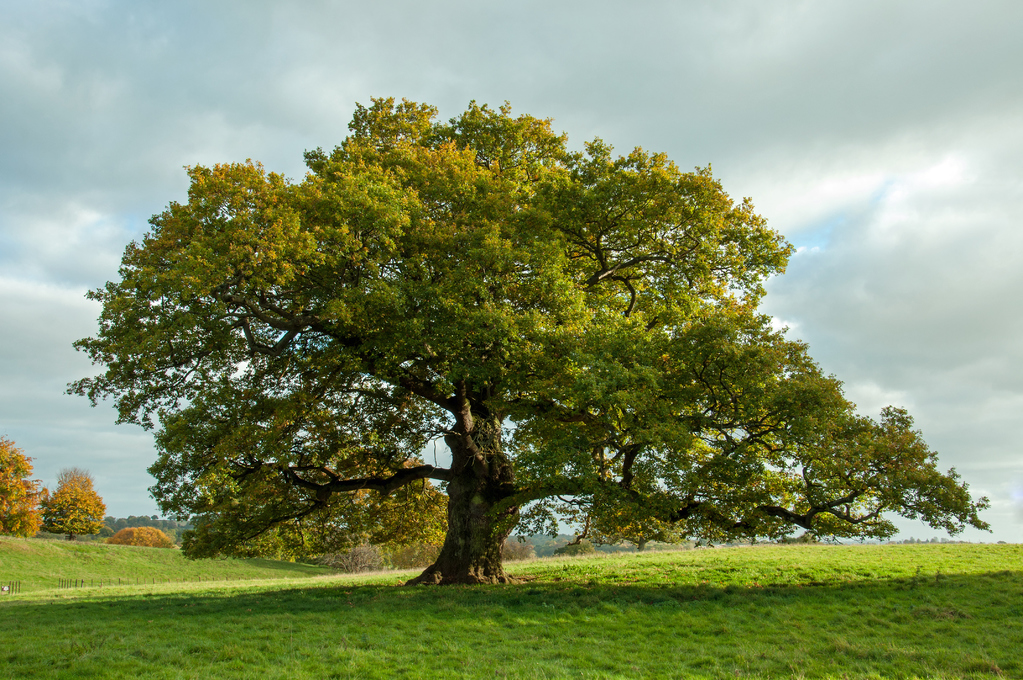
\includegraphics[width=0.3\textwidth]{pictures/drzewo.jpeg}
    \caption{\textbf{This is a tree}}
    \label{fig:tree}
\end{figure}

This is the table:
\begin{table}[h]
\centering
\begin{tabular}{lllll}
+ & 1 & 2 & 3 & 4 \\
1 & 2 & 3 & 4 & 5 \\
2 & 3 & 4 & 5 & 6 \\
3 & 4 & 5 & 6 & 7
\end{tabular}
\end{table}

\textbf{This is an unnumbered list:}
\begin{itemize}
    \item one
    \item two
    \item three
\end{itemize}

\textbf{This is a numbered list: }  
\begin{enumerate}
    \item one
    \item two
    \item three
\end{enumerate}

\section*{Paragraph}

\begin{flushright}
\textbf{\textit{This is text contained in the first paragraph. This is text contained in the first paragraph. This is text contained in the first paragraph.}}
\end{flushright}

\textbf{\textit{This is text contained in the first paragraph. This is text contained in the first paragraph. This is text contained in the first paragraph.}}